\documentclass[10pt,a4paper]{article}

\usepackage[left=1.5cm, right=1.5cm, top=1.5cm, bottom=1.5cm]{geometry}
\usepackage[utf8]{inputenc}
\usepackage[english]{babel}
\usepackage{enumitem}
\usepackage{hyperref}
\usepackage{titlesec}
\usepackage{graphicx}
\usepackage{wrapfig}
\usepackage{xcolor}

\newcommand{\resumeItem}[5]{
    \noindent \textbf{#1} \hfill \textbf{#2}
    \ifboolexpr{test {\ifstrempty{#3}} and test {\ifstrempty{#4}}}{}{
        \\
        \textit{#3} \hfill #4
    }
    \ifstrempty{#5}{}{
        \begin{itemize}[noitemsep,topsep=0pt,leftmargin=1.5em]
            #5
        \end{itemize}
    }
    \vspace{1em}
}

\titleformat{\section}{\large\bfseries\uppercase}{}{0em}{}[\titlerule]
\titlespacing{\section}{0pt}{10pt}{5pt}

\pagestyle{empty}

\begin{document}

\noindent
\begin{minipage}[c]{0.82\textwidth}
    {\Huge \textbf{Eliseo Martelli}} \\[4pt]
    \textbf{Researcher \& Software Developer} \\[4pt]
    Via Carrù, 9, Torino (TO) 10141, Italy \\
    +39 392 504 9974 $\cdot$ \href{mailto:me@eliseomartelli.it}{me@eliseomartelli.it} \\
    \href{https://eliseomartelli.it}{https://eliseomartelli.it} $\cdot$ \href{https://github.com/eliseomartelli}{github.com/eliseomartelli}
\end{minipage}%
\begin{minipage}[c]{0.18\textwidth}
    \begin{flushright}
        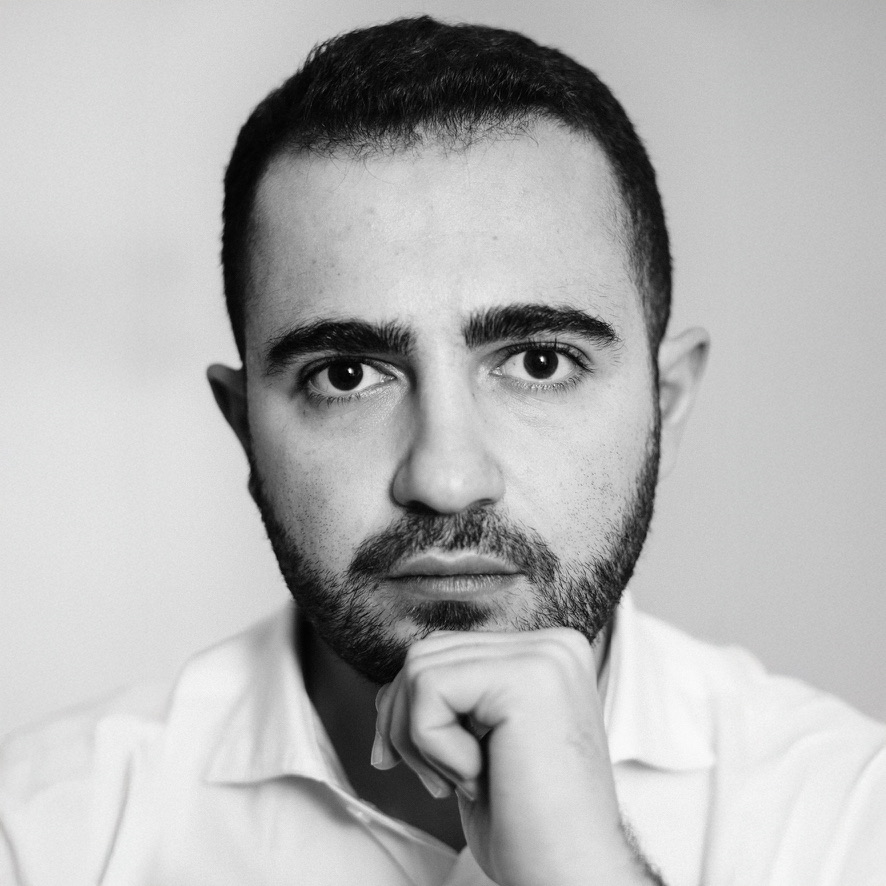
\includegraphics[width=3cm, height=3.8cm, keepaspectratio]{portrait.jpg}
    \end{flushright}
\end{minipage}

\section{Work Experience}

\resumeItem{Researcher \& Software Developer}{2024 -- 2026}{Consortium GARR}{Rome, Italy}{
    \item Developed a Reproducible Bioinformatics Environment Platform and a distributed computation platform.
    \item Architected a C++ annotation library to automate code conversion for Fully Homomorphic Encryption (FHE) calculations.
    \item Responsible for Quality Assurance \& Testing.
}

\resumeItem{Software Developer}{2024}{Federazione Gomma Plastica}{Milan, Italy}{
    \item Developed and deployed the official tire-check application for Polizia Stradale used on service tablets during the 2025 national safety campaign.
    \item Built the Android Application, Authentication Platform, and Management Web Application.
    \item Managed software deployment using Docker.
}

\resumeItem{Open Source Software Contributor}{Ongoing}{}{}{
    \item Contributing to Internet of Things platforms and software libraries to enhance developer experience.
}

\resumeItem{Independent Fullstack Developer}{2014 -- 2024}{}{}{
    \item End-to-end development of Android applications (Java/Kotlin) with custom Python/PHP backends, implementing local storage and real-time cloud synchronization.
}

\resumeItem{Independent Android Developer}{2014 -- 2019}{}{}{
    \item Developed and tested large Android codebases (Java \& Kotlin).
    \item Handled product marketing and design.
}

\resumeItem{Network Technician}{2017 -- 2018}{Dedalonet S.r.l.}{Lanciano (CH), Italy}{
    \item Network analysis and implementation for third parties.
    \item Software development for process automation and embedded devices.
}

\section{Education}

\noindent \textbf{Master Degree in Computer Science} \hfill \textbf{2023 -- Ongoing} \\
\textit{Università degli Studi di Torino} \\
\textbf{Thesis}: \textit{ongoing}

\noindent \textbf{Bachelor Degree in Computer Science} \hfill \textbf{2019 -- 2023} \\
\textit{Università degli Studi di Torino} \\
\textbf{Thesis}: Edge-computing workload management in heterogeneous environments

\section{Technical Skills}

\noindent
\begin{tabular}{@{}ll}
\textbf{Languages:} & Python, Go, Java, Kotlin, Swift, Javascript, Typescript, C, Dart \\
\textbf{Protocols \& APIs:} & XML, JSON, REST, RPC, APIs, GraphQL \\
\textbf{Infrastructure:} & Docker, Podman, LibVirt, VMWare, Proxmox, Xen \\
\textbf{Databases:} & MySQL / MariaDB, PostgreSQL, SQLite, MongoDB \\
\textbf{Tools:} & Git, Vim, GitHub, Xcode, Android Studio, Microsoft Office, Adobe Creative Suite \\
\textbf{Other:} & Visual storytelling, Graphic content creation
\end{tabular}

\section{Languages}
\noindent
\textbf{Italian:} Native \quad $\cdot$ \quad
\textbf{English:} Proficient \quad $\cdot$ \quad
\textbf{Spanish:} Basic

\section{Additional Information}
\noindent
\textbf{Driving License:} B

\end{document}
